% Created 2014-05-27 Tue 09:33
\documentclass[bigger, presentation]{beamer}
\usepackage[utf8]{inputenc}
\usepackage[T1]{fontenc}
\usepackage{fixltx2e}
\usepackage{graphicx}
\usepackage{longtable}
\usepackage{float}
\usepackage{wrapfig}
\usepackage{soul}
\usepackage{textcomp}
\usepackage{marvosym}
\usepackage{wasysym}
\usepackage{latexsym}
\usepackage{amssymb}
\usepackage{hyperref}
\tolerance=1000
\usepackage{minted}
\usetheme{Frankfurt}   
\usecolortheme[RGB={0,104,139}]{structure}%deepskyblue
\usefonttheme{serif}  % or try serif, structurebold, ...
\setbeamertemplate{navigation symbols}[horizontal]
\setbeamertemplate{caption}[numbered]
\useinnertheme{rounded}
\setbeamercovered{transparent}
\usepackage{pgfpages}
\pgfpagesuselayout{resize to}[physical paper width=8in, physical paper height=6in]
\logo{
\includegraphics[height=1cm,width=1cm]{iitb-logo.jpeg}}
\usepackage{array}
\usepackage{graphicx}
\usepackage{hyperref}
\usepackage[english]{babel}
\usepackage{pxfonts}
\usepackage{listings}
\lstset{numbers=left,numbersep=6pt,numberstyle=\tiny,showstringspaces=false,aboveskip=-50pt,frame=leftline,keywordstyle=\color{black},commentstyle=\color{orange},stringstyle=\color{black},}
\date{today}
\subtitle{because we like silly names}
\institute{Indian Institute of Technology, Bombay}
\providecommand{\alert}[1]{\textbf{#1}}

\title{git}
\author{Sachin}
\date{\today}
\hypersetup{
  pdfkeywords={git, version control},
  pdfsubject={my first presentation made in org mode},
  pdfcreator={Emacs Org-mode version 7.9.3f}}

\begin{document}

\maketitle

\section{Introduction}
\label{sec-1}
\begin{frame}
\frametitle{What is git?}
\label{sec-1-1}

\begin{quote}
A programs that remembers the changes in your file(s)
\end{quote}
\end{frame}
\begin{frame}
\frametitle{Other version control systems}
\label{sec-1-2}

\begin{itemize}
\item Mercurial(\texttt{hg})
\item Subversion Control(\texttt{svn})
\item bazaar(\texttt{bzr})
\end{itemize}
\end{frame}
\section{Summary}
\label{sec-2}
\begin{frame}
\frametitle{Why should I use git?}
\label{sec-2-1}

\begin{itemize}
\item Once you get familiar it will be a part of you life.
\item Cleaner approach to file management
\end{itemize}
\end{frame}
\begin{frame}
\frametitle{Usefulness}
\label{sec-2-2}

\begin{quote}
I'm no coder or a developer, can I use \textbf{git}?
\end{quote}

     
\end{frame}
\begin{frame}
\frametitle{Basic concept}
\label{sec-2-3}

   \begin{figure}[htb]
   \centering
   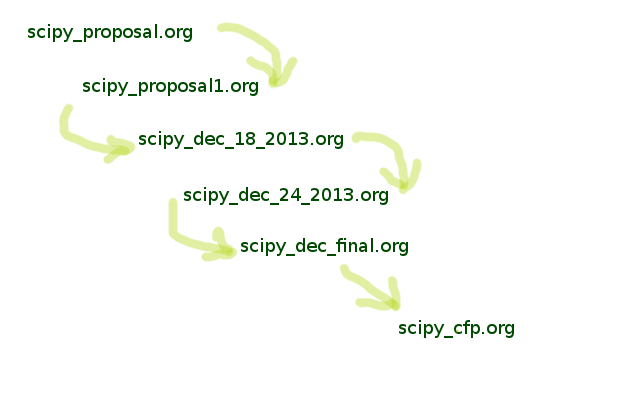
\includegraphics[width=9cm,angle=0]{./concept.png}
   \caption{\label{fig:life-of-file}life of a file}
   \end{figure}
\end{frame}
\section{Install}
\label{sec-3}
\begin{frame}[fragile]
\frametitle{Installing \texttt{git}}
\label{sec-3-1}


   \emph{Ubuntu(or Debian)}

\begin{minted}[]{sh}
sudo apt-get install git
\end{minted}

   \emph{From source - Download and compile/install}

\begin{minted}[]{html}
http://git-scm.com/downloads
\end{minted}
\end{frame}
\section{Setup}
\label{sec-4}
\begin{frame}[fragile]
\frametitle{Basic setup}
\label{sec-4-1}

   
   \emph{Your name}

\begin{minted}[]{sh}
git config --global user.name "Sachin"
\end{minted}

   \emph{Your Email}

\begin{minted}[]{sh}
git config --global user.email "isachin@iitb.ac.in"
\end{minted}
\end{frame}
\section{Hands on}
\label{sec-5}
\begin{frame}[fragile]
\frametitle{Make a project}
\label{sec-5-1}

   \emph{Make a directory/folder to store your file(s)}
     

\begin{minted}[]{sh}
mkdir octo
\end{minted}
\end{frame}
\begin{frame}[fragile]
\frametitle{Tell git to manage it}
\label{sec-5-2}


   \emph{Initialize git}


\begin{minted}[]{sh}
git init
\end{minted}

   
   \emph{at this time I want to know the status of my project}


\begin{minted}[]{sh}
git status
\end{minted}
\end{frame}
\begin{frame}[fragile]
\frametitle{Add file to your project}
\label{sec-5-3}


\begin{minted}[]{sh}
git add <FILE NAME>
\end{minted}

   \emph{for files with similar extensions}

\begin{minted}[]{sh}
git add *.txt
\end{minted}

   \emph{to add everything}

\begin{minted}[]{sh}
git add .
\end{minted}
\end{frame}
\begin{frame}[fragile]
\frametitle{Check status of your project}
\label{sec-5-4}



\begin{minted}[]{sh}
git status
\end{minted}
\end{frame}
\begin{frame}[fragile]
\frametitle{Commit it if your are happy :D}
\label{sec-5-5}



\begin{minted}[]{sh}
git commit -m "My message"
\end{minted}
\end{frame}
\section{diff}
\label{sec-6}
\begin{frame}[fragile]
\frametitle{See changes w.r.t last commit}
\label{sec-6-1}

   

\begin{minted}[]{sh}
git diff
\end{minted}

   \emph{Difference w.r.t file}

\begin{minted}[]{sh}
git diff <FILENAME>
\end{minted}
\end{frame}
\section{Update}
\label{sec-7}
\begin{frame}[fragile]
\frametitle{Update modified file(s)}
\label{sec-7-1}

   
   \emph{to update already committed file}

\begin{minted}[]{sh}
git add -u
\end{minted}

   (\emph{do some more commits})
\end{frame}
\section{Log}
\label{sec-8}
\begin{frame}[fragile]
\frametitle{View commits}
\label{sec-8-1}


\begin{minted}[]{sh}
git log
\end{minted}


\begin{minted}[]{sh}
git log --oneline
\end{minted}


\begin{minted}[]{sh}
git log --graph --decorate --oneline
\end{minted}
\end{frame}
\section{Reset/Reflog/Revert}
\label{sec-9}
\begin{frame}[fragile]
\frametitle{Get back to old commit}
\label{sec-9-1}
\begin{itemize}

\item With no history\\
\label{sec-9-1-1}%
\begin{minted}[]{sh}
git reset --hard <COMMIT HASH>
\end{minted}

\end{itemize} % ends low level
\end{frame}
\section{GitHub}
\label{sec-10}
\begin{frame}
\frametitle{Hosting your code}
\label{sec-10-1}



  \begin{figure}[htb]
  \centering
  
\includegraphics[width=10cm,angle=0]{./github.png}
  \caption{\label{fig:GitHub}GitHub}
  \end{figure}
\end{frame}
\section{Branch}
\label{sec-11}
\begin{frame}
\frametitle{Git branch: What is that?}
\label{sec-11-1}



  \begin{figure}[htb]
  \centering
  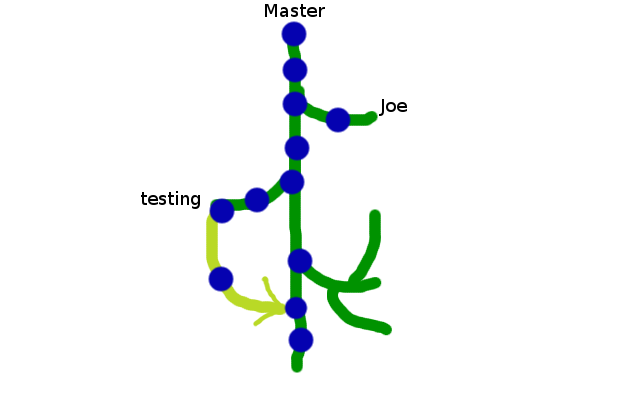
\includegraphics[width=10cm,angle=0]{./branch.png}
  \caption{\label{fig:branch}Git branches}
  \end{figure}
\end{frame}
\section{Hosting}
\label{sec-12}
\begin{frame}
\begin{block}{Hosting sites}
\label{sec-12-1-1}

\begin{itemize}
\item github.com
\item gitlab.com
\item bitbucket.org
\end{itemize}
     
\end{block}
\end{frame}
\section{Question}
\label{sec-13}
\begin{frame}[fragile]

   
\includegraphics[width=5cm,angle=0]{./questions.png}
   

\begin{minted}[]{sh}
isachin@iitb.ac.in
\end{minted}
\end{frame}
\section{Reference \& links}
\label{sec-14}
\begin{frame}
\begin{block}{Reference}
\label{sec-14-1-1}

\begin{itemize}
\item \emph{Pro Git}
\end{itemize}
\end{block}
\begin{block}{Links}
\label{sec-14-1-2}

\begin{itemize}
\item \href{http://www.emacswiki.org/emacs/}{http://git-scm.com/}
\end{itemize}
\end{block}
\end{frame}

\end{document}
